\subsection{2018 Free-Response Questions}
Questions 1 and 2 are part of the same section and are allotted 30 minutes for completion with the aid of a graphing calculator.
Question 3 through 6 are part of the same section are allotted 1 hour for completion without the aid of a graphing calculator.

\begin{enumerate}
	\item People enter a line for an escalator at  rate modeled by the function $r$ given by
	\begin{equation*}
		r(t) = \begin{cases}
			44\left(\frac{t}{100}\right)^3\left(1-\frac{t}{300}\right)^7 & \text{for } 0 \leq t \leq 300 \\
			0 & \text{for } t > 300,
		\end{cases}
	\end{equation*}
	where $r(t)$ is measured in people per scond and $t$ is measured in seconds.
	As people get on to the escalator, they exit the line at a rate of 0.7 person per second,
	There are 20 people in line at time $t=0$.
	\begin{enumerate}
		\item How many people entered the line for the escalator during the time interval $0 \leq t \leq 300$?
		\item During the time interval $0 \leq t \leq 300$, there are always people in line for the escalator.
			How many people are in line at time $t=300$?
		\item For time $t > 300$, what is the first time $t$ that there are no people in line for the escalator?
		\item For time $0 \leq t \leq 300$, at what time $t$ is the number of people in line at a minimum?
			To the nearest whole number, find the number of people in line at this time.
			Justify your answer.
	\end{enumerate}

	\item Researchers on a boat are investigating plankton cells in a sea.
		At a depth of $h$ meters, the density of plankton cells, in millions of cells per cubic meter, is modeled by $p(h) = 0.2h^2e^{-0.0025h^2}$ for $0 \leq h \leq 30$ and is modeled by $f(h)$ for $h\geq 30$.
		The continuous function $f$ is not explicitly given.
		\begin{enumerate}
			\item Find $p^\prime(25)$.
				Using correct units, interpret the meaning of $p^\prime(25)$ in the context of the problem.
			\item Consider a vertical column of water in this sea with horizontal cross sections of constant area 3 square meters.
				To the nearest million, how many plankton cells are in this column of water between $h=0$ and $h=30$ meters?
			\item There is a function $u$ such that $0 \leq f(h) \leq u(h)$ for all $h \geq 30$ and $\int_{30}^{\infty}{u(h)\d{h}} = 105$.
				The column of water in part (b) is $K$ meters deep, where $K > 30$.
				Write an expression involving one or more integrals that gives the number of plankton cells in the entire column.
				Explain why this number of plankton cells is less than or equal to 2000 million.
			\item The boat is moving on the surface of the sea.
				At time $t \geq 0$, the position of the boat is $(x(t),y(t))$, where $x^\prime(t) = 662\sin{(5t)}$ and $y^\prime(t)=880\cos{(6t)}$.
				Time $t$ is measured in hours, and $x(t)$ and $y(t)$ are measured in meters.
				Find the total distance traveled by the boat over the time interval $0 \leq t \leq 1$.
		\end{enumerate}
	
		\begin{figure}[H]
			\label{2018_3}
			\centering
			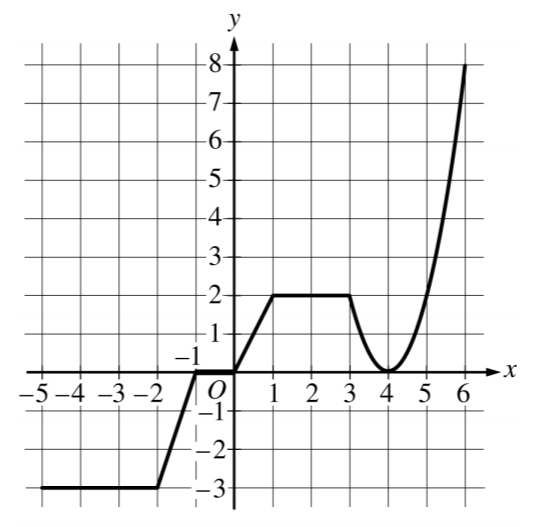
\includegraphics[width=0.5\textwidth]{./additional_materials/2018_3.png}
			\caption{\hyperref{https://apcentral.collegeboard.org/pdf/ap18-frq-calculus-bc.pdf}{}{}{AP Calculus BC 2018 Exam Free-Response Question 3, Graph of $g$}}
		\end{figure}
	
	\item
		The graph of the continuous function $g$, the derivative of a function $f$, is shown above.
		The function $g$ is piecewise linear for $-5 \leq x < 3$ and $g(x)=2(x-4)^2$ for $3 \leq x \leq 6$.
		\begin{enumerate}
			\item If $f(1)=3$, what is the value of $f(-5)$?
			\item Evaluate $\int_{1}^{6}{g(x)\d{x}}$.
			\item For $-5 < x < 6$, on what open intervals, if any, is the graph of $f$ both increasing and concave up?
				Give a reason for your answer.
			\item Find the $x$-coordinate of each point of inflection of the graph of $f$.
				Give a reason for your answer.
		\end{enumerate}
	
		\begin{table}[H]
			\begin{center}
				\begin{tabular}{|c||c|c|c|c|c|}
					\hline
					$t$ (years) & 2 & 3 & 5 & 7 & 10 \\
					\hline
					$H(t)$ (meters) & 1.5 & 2 & 6 & 11 & 15 \\
					\hline
				\end{tabular}
			\end{center}
		\end{table}
	
	\item The height of a tree at time $t$ is given by a twice-differentiable function $H$, where $H(t)$ is measured in meters and $t$ is measured in years.
		Selected values of $H(t)$ are given in the table above.
		\begin{enumerate}
			\item Use the data in the table to estimate $H^\prime(6)$.
				Using correct units, interpret the meaning of $H^\prime(6)$ in the context of the problem.
			\item Explain why there must be at least one time $t$, for $2 \leq t \leq 10$ such that $H^\prime(t) = 2$.
			\item Use a trapezoidal sum with 4 subintervals indicated by the data in the table to approximate the average height of the tree over the time interval $2 \leq 2 \leq 10$.
			\item The height of the tree, in meters, can also be modeled by the function $G$, given by $G(x)=\frac{100x}{1+x}$, where $x$ is the diameter of the base of the tree, in meters.
				When the tree is 50 meters tall, the diameter of the base of the tree is increasing at a rate of 0.03 meters per year.
				According to this model, what is the rate of the change of the height of the tree with respect to time, in meters per year, at the time when the tree is 50 meters tall?
		\end{enumerate}
	
	\begin{figure}[H]
		\label{2018_5}
		\centering
		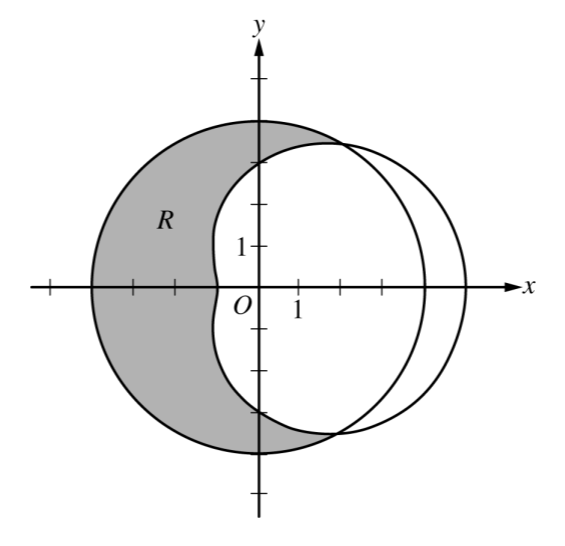
\includegraphics[width=0.5\textwidth]{./additional_materials/2018_5.png}
		\caption{\hyperref{https://apcentral.collegeboard.org/pdf/ap18-frq-calculus-bc.pdf}{}{}{AP Calculus BC 2018 Exam Free-Response Question 5}}
	\end{figure}
	
	\item The graph of the polar curves $r=4$ and $r=3+2\cos{\theta}$ are shown in the figure above.
		The curves intersect at $\theta = \frac{\pi}{3}$ and $\theta = \frac{5\pi}{3}$.
		\begin{enumerate}
			\item Let $R$ be the shaded region inside the graph of $r=4$ and outside the graph of $r=3+2\cos{\theta}$, as shown in the figure above.
				Write an expression involving an integral for the area of $R$.
			\item Find the slope of the line tangent to the graph $r=3+2\cos{\theta}$ at $\theta = \frac{\pi}{2}$.
			\item A particle moves along the portion of the curve  $r=3+2\cos{\theta}$ for $0 < \theta < \frac{\pi}{2}$.
				The particle moves in such a way that the distance between the particle and the origin increases at a constant rate of 3 units per second.
				Find the rate at which the angle $\theta$ changes with respect to time at the instant when the position of the particle corresponds to $\theta = \frac{\pi}{3}$.
				Indicate units of measure.
		\end{enumerate}
	
	\item The Maclaurin series for $\ln{(1+x)}$ is given by
		\begin{equation*}
			x - \frac{x^2}{2} + \frac{x^3}{3} - \frac{x^4}{4} + \ldots + (-1)^{n+1}\frac{x^n}{n} + \ldots .
		\end{equation*}
		On its interval of convergence, this series converges to $\ln{(1+x)}$.
		Let $f$ be a function defined by $f(x) = x\ln{\left(1+\frac{x}{3}\right)}$.
		\begin{enumerate}
			\item Write the first four nonzero erms and the general term of the Maclaurin series for $f$.
			\item Determine the interval of convergence for $f$.
				Show the work that leads to your answer.
			\item Let $P_4(x)$ be the fourth-degree Taylor polynomial for $f$ about $x=0$.
				Use the alternating series estimation bound to find an upper bound for $\abs{P_4(2)-f(2)}$.
		\end{enumerate}
	
\end{enumerate}